\chapter{Operations and Logistics}

%This chapter will outline the operational and logistical process involved in making HUGO operational once the design and certification process is completed. The operations plan of HUGO will describe the usage practices and mission objectives, this section covers the concept, mission timeline and phases, constraints on operation, maintenance provisions and future scalability. The logistics section will include analysis on budgts such as ground personnel required, deployment logistics, location and facility and a consumable estimations (spare parts, supply chain, etc.)

This Chapter presents the operational and logistical framework required to bring HUGO into service following completion of the design and certification process. In \autoref{sec:operations}, the intended use of the system is described, covering the concept of operations, mission objectives, mission phases, operational constraints, and maintenance provisions. \autoref{sec:logistics} addresses the supporting resources needed for sustained operation, including: ground personnel, deployment logistics, facility and location requirements, consumables, spare parts, and supply-chain considerations. Finally, \autoref{sec:scalability} explores the potential of future scalability of HUGO.
%This combined analysis establishes how HUGO can be practically deployed, supported, and maintained throughout its operational life.

\begin{comment}

Devide the chapter into 2 parts, operation and logistics

Operation
Operational and Logistical Analysis

1. Operational Concept - O
2. Mission Timeline and Phases - O
3. Required Personnel and Responsibilities - L
4. Ground Support and Deployment Logistics - L
5. Operational Constraints - O
6. Maintenance and Turnaround - exclude for now or it can be implemented later - O
7. Consumables, Spare Parts and Supply Chain - not applicable or write only a short part -L

8. Cost of Operation - detailed in the TAM SAM SOM
9. Contingency Procedures  - covered in the previous section
10. Regulatory and Safety Considerations - covered by certification and risk management part (included into the airport fees)

11. Scalability of Operations - to be determined and written -O 

\end{comment}

\todo[inline]{!!!ALL OF BELOW SECTIONS HAVE TO BE EXPANDED ON !!!!!}

\section{Operations}
\label{sec:operations}
This Section contains a detailed description of the intended operations for HUGO, incl. an overview of the system users, testing location and conditions, mission phases, an approximate timeline. A brief discussion is additionally dedicated to operational constraints and maintenance procedures to ensure successful continuous operation of the UAV.

\subsection{High-level Mission Description}
The main objective HUGO is to simulate high subsonic flight of commercial aircraft, while simultaneously implementing AFS and GLA and recording relevant flight parameters. A mission is considered as successful if all the below apply:
\begin{enumerate}
    \item The speed of Mach 0.75 was achieved and maintained for 5 consecutive minutes of straight flight.
    \item All control systems required for the specific test were activated and performed their duties without error.
    \item The flight data was successfully recorded, downloaded and provided to the customer.
\end{enumerate}

Market analysis and segmentation performed in the previous design phases highlighted four main sectors in which potential customers can be identified: universities and academic laboratories, research centres, aerospace companies, and defence\footnote{\label{url:baseline_report}\href{https://github.com/Teo-Cokonaj/DSE-28/blob/main/docs/Projects/DSE_Group_28_Baseline_Report.pdf}{HUGO Baseline Report} (accessed on 08.05.2026)}. Moreover, the Netherlands was identified as the beachhead market. Therefore, a suitable aerodrome was found in TBD.

\todo[inline]{A description of the test site and operational volume goes here. Also, describe the conditions and constraints related to the operations.}

\todo[inline]{Include a map of operations if possible, once more information is available. Hopefully NLR will reply. Otherwise we ball with Den Helder.}

\begin{comment}
\begin{itemize}
\item Who uses the system?
\item Where it operates?
\item Under what conditions it operates?
\item What the mission objective is?
\item What success looks like?
\item What constraints affect operation?
\end{itemize}
\end{comment}


\subsection{Mission Phase and Timeline}
A reference test day for HUGO is assumed to include four
test flights for 100 operational days per year\footref{url:baseline_report}. Four main phases were identified for a test day: transport to test site, followed by pre-flight, in-flight, and post-flight operations. These shall now be evaluated in more detail.


\subsubsection{Transport to Test Site}
The day before a test flight is scheduled, the Terminal Aerodrome Forecast (TAF) shall be consulted to ensure that departure will be possible. In case of adverse weather prediction, the test day (or part of it) shall be cancelled and the customer shall be informed. 

In case the weather prediction allows for a successful take-off, the test day shall proceed according to schedule. If the test requires parts provided by the client to be mounted onto HUGO, these shall be integrated in the hangar, before proceeding onto the airfield. The ground station and fuel required for the flight shall also be transported onto the airfield.

\subsubsection{Pre-Flight Operations}
This subsection defines the pre-flight operations required before HUGO can proceed to the take-off checklist. The pre-flight phase begins once HUGO is unloaded from the transportation unit and ends when the aircraft is powered on, all checks are performed, and fuel is loaded on board. The objective of this phase is to verify that the mission plan, operating environment, ground support equipment, aircraft configuration, and safety provisions are suitable for the intended mission.

An overview of the pre-flight steps is provided in \autoref{fig:pre-flight_checklist}. Once HUGO is unloaded, the mission plan is reviewed, and NOTAMs are checked for restrictions and updates. If a go or conditional go is given, HUGO can be configured for the mission profile, and the crew briefing and preparation checklists can be done. Otherwise, the test shall be cancelled or delayed. Once all preparation steps are checked and recorded, HUGO can be considered as ready to fly, and the test personnel can proceed to the in-flight phase of the mission.


\begin{comment}
The following steps will be considered in the pre-flight preparation:

\begin{enumerate}
    \item Unload HUGO from transportation unit,
    \item Mission Plan Review,
    \item NOTAM check for restrictions and updates,
    \item Final TAF check for weather details (go/no-go/conditional go),
    \item Configure HUGO for the Mission profile,
    \item Crew Briefing,
    \item Configure the ground station equipment,
    \item External inspection of HUGO (walk-around),
    \item System checks (using pre-flight checklists),
    \item Calibrate sensors,
    \item Load fuel onboard HUGO.
\end{enumerate}
\end{comment}
\begin{figure}[H]
    \centering
    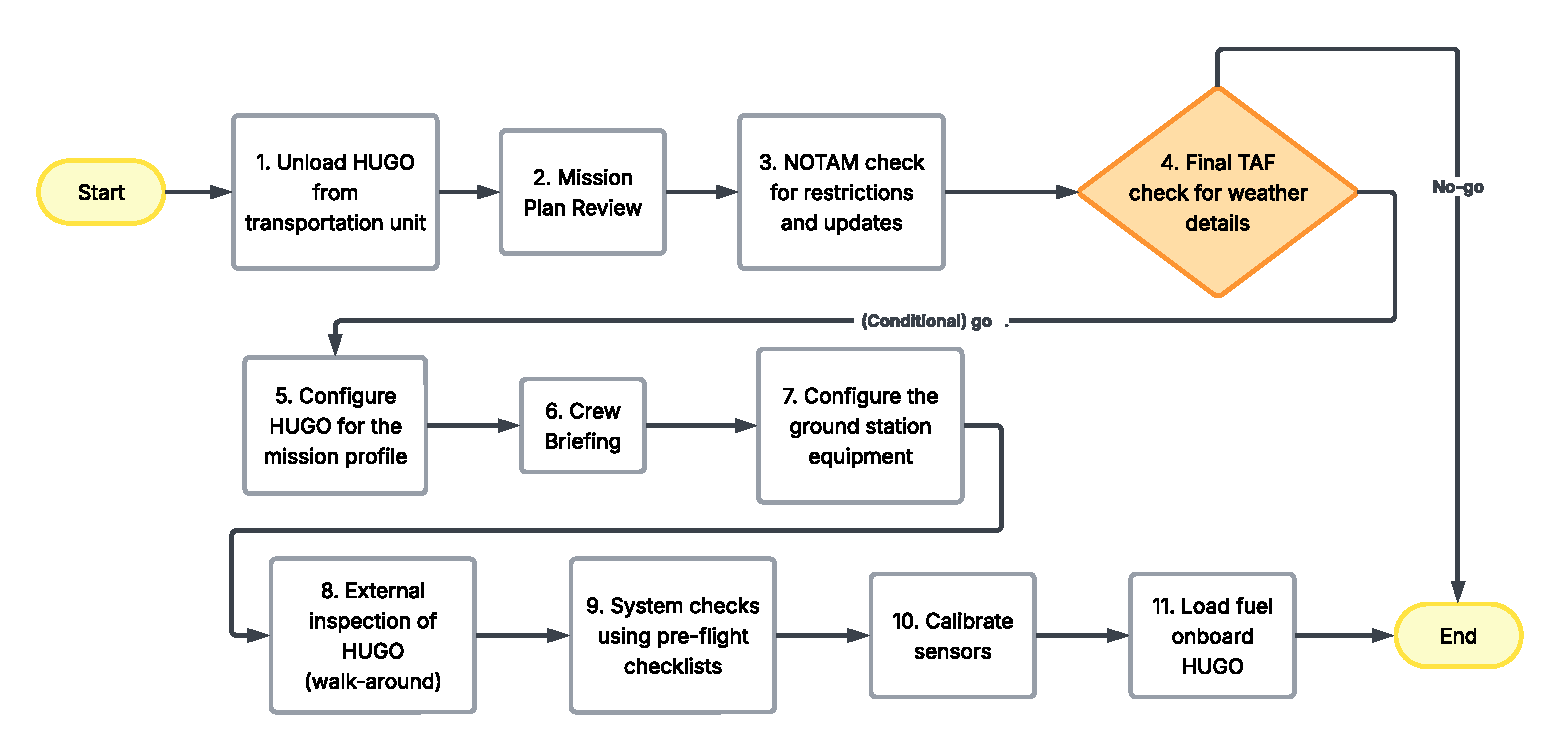
\includegraphics[width=1\linewidth]{figures/pre_flight_checklist.pdf}
    \caption{HUGO Pre-Flight Operations}
    \label{fig:pre-flight_checklist}
\end{figure}


\subsubsection{In-Flight Operations}
Once all necessary pre-flight checklists are done and ATC clearance for take-off is obtained, HUGO will be able to enter the next mission phase. This stage of operations begins when the engines are turned on prior to take-off and ends when they are turned off post-landing. The objective of this mission phase is to perform the test and obtain measurements requested by the customer. 

An overview of the expected in-flight operations is provided in \autoref{fig:in-flight_ops}. After engine turn-on, HUGO will taxi onto the runway and take-off. After climbing to test altitude and reaching test area, it shall accelerate to Mach 0.75 and perform the 5 min test, while transmitting measurement data back to the ground station. Subsequently, it shall be ordered to decelerate, return to the airfield, and perform a landing. It is expected that holding or go-around manoeuvres may be necessary prior to landing. These scenarios will be included in the fuel budget.

\begin{comment}
\begin{enumerate}
    \item Engine turn-on,
    \item Taxi to runway,
    \item Perform take-off,
    \item Climb to test altitude and reach test area,
    \item Perform test (constant monitoring from ground: continue/hold/abort test),
    \item Return to airfield,
    \item Perform landing approach (or hold if instructed by ATC),
    \item Perform a go-around (if necessary),
    \item Perform landing,
    \item Taxi from runway,
    \item Engine shut-off
\end{enumerate}
\end{comment}

\begin{figure}[H]
    \centering
    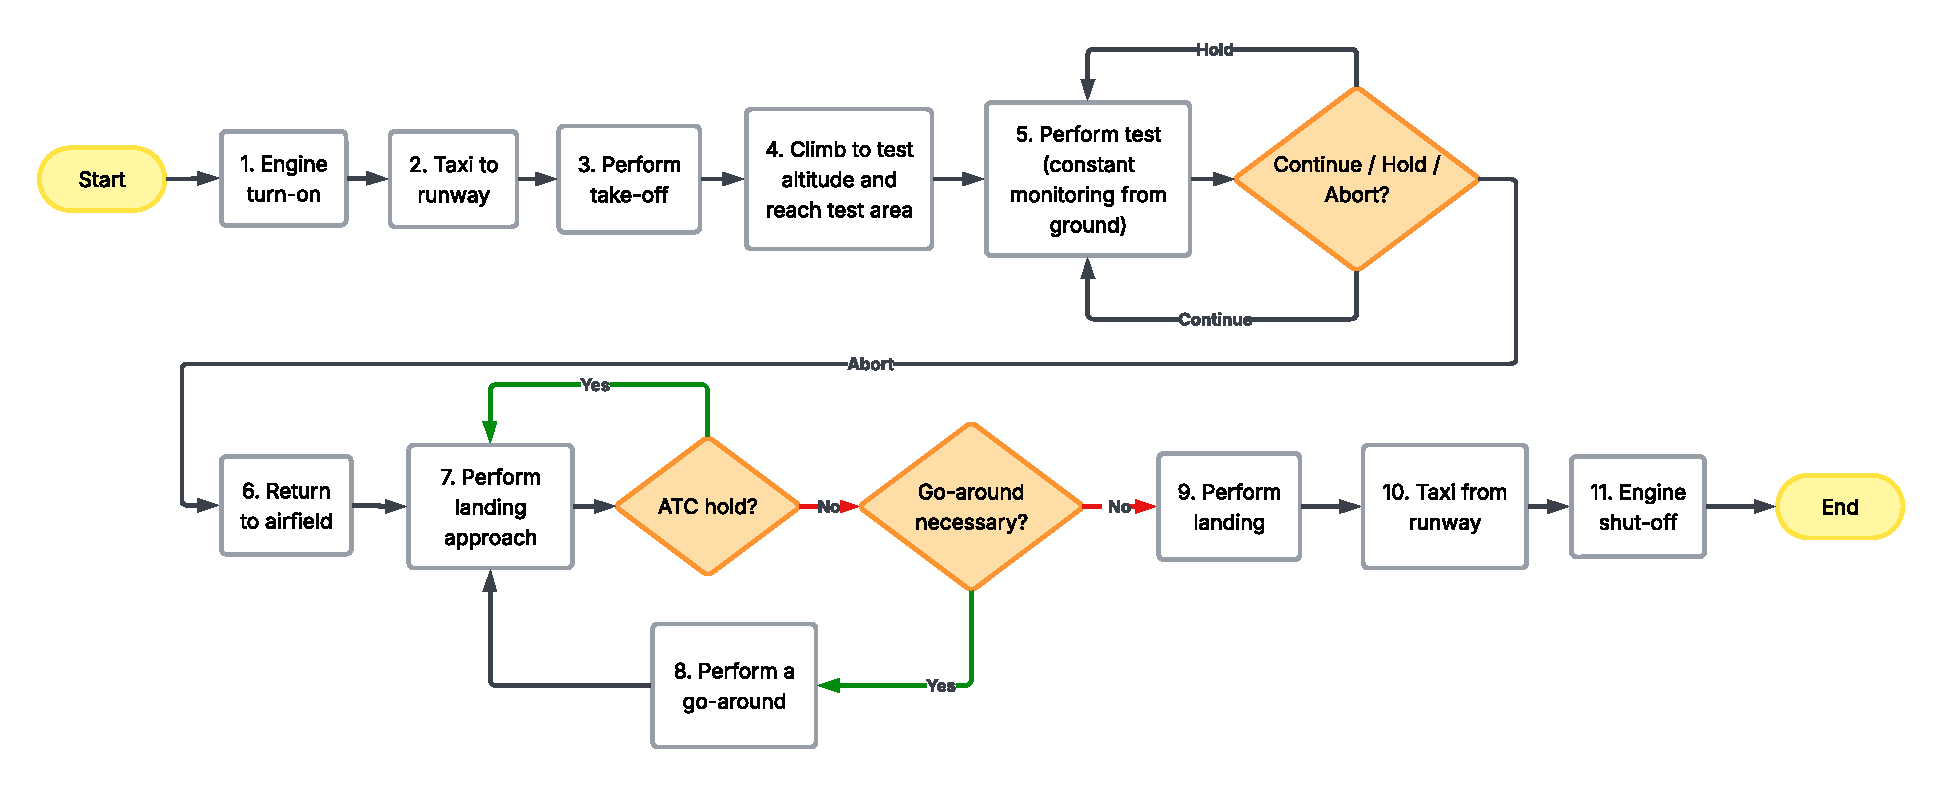
\includegraphics[width=1\linewidth]{figures/in-flight_checklist.pdf}
    \caption{HUGO In-Flight Operations}
    \label{fig:in-flight_ops}
\end{figure}

\subsubsection{Post-Flight Operations}
After the UAV is on the ground, the post-flight data extraction and operations can commence. At this stage of the operation process, there are 2 possible scenatios that can take place depending on the mission profile of the day. HUGO can either undergo dissabele and reclaim procedure or can be prepared for a follow up flight.
If the UAV is set to go for another test flight, the following check will be performed:

\begin{enumerate}
    \item Download data from the previous test
    \item Perform check the internal and external systems of the UAV to ensure no problem developed
    \item Perform visually inspect the fuselage for damage
    \item Refill the tanks of HUGO
    \item Perform in-flight operation plan 
\end{enumerate}

Once HUGO has finished with the tests planned for that fly day, it will undergo the following steps of recall and disassembly, at the end marking the end of the test-flight day. The following procedure list will be followed by the ground crew:

\begin{enumerate}
    \item Download data from the test flight
    \item Perform a check of the onboard systems to check that no system problems exist
    \item Turn off power supply
    \item Perform visual inspection of the fuselage to check for damage
    \item Perform maintenance if required
    \item Perform debriding of the flight day
    \item Perform disassembly of HUGO
    \item Load the equipment into the van
    \item End the flight day
\end{enumerate}

The completion of the post-flight operations checklist marks the end of the flight day. If any unforeseen events, anomalies, or deviations occurred during the mission, the flight day shall be followed by an additional debriefing and the completion of the required documentation.

\subsection{Operational constrains}
this one will be strongly paired with the EASA restrictions and airfield specifications

\subsection{Maintenance}

\section{Logistics}
\label{sec:logistics}

\subsection{Personal Required for Operation}

\subsection{Storage Hangar}

We are going with Den Helder no comment here

this is more a section where we decide if it is more feasible to have hugo stored in a warehouse and perform changes on it there or have a hangar rented at the airfield
Use as ref 3 airports and perharps one from outside of NL
Statement- we have to look as well if the airport will allow us to performa operations, waiting time and so on

\subsection{Airfield and Ground Support}
Include the operational constraints and the requirements from EASA as well as the costs and the needed dimensions
Apply for ATC approval, ATC location and the flight plan/plans for the route.
We will be fling above water in a restricted region as per instructions and baseline info 
\subsection{Parts and Supply Chain}



\section{Scalability of Operation}
\label{sec:scalability}

Bullshit based on the money we get and expected probability of expansion